\documentclass{sigchi}

% Use this section to set the ACM copyright statement (e.g. for
% preprints).  Consult the conference website for the camera-ready
% copyright statement.

% Copyright
\CopyrightYear{2016}
%\setcopyright{acmcopyright}
\setcopyright{acmlicensed}
%\setcopyright{rightsretained}
%\setcopyright{usgov}
%\setcopyright{usgovmixed}
%\setcopyright{cagov}
%\setcopyright{cagovmixed}
% DOI
\doi{http://dx.doi.org/10.475/123_4}
% ISBN
\isbn{123-4567-24-567/08/06}
%Conference
\conferenceinfo{CHI'16,}{May 07--12, 2016, San Jose, CA, USA}
%Price
\acmPrice{\$15.00}

% Use this command to override the default ACM copyright statement
% (e.g. for preprints).  Consult the conference website for the
% camera-ready copyright statement.

%% HOW TO OVERRIDE THE DEFAULT COPYRIGHT STRIP --
%% Please note you need to make sure the copy for your specific
%% license is used here!
 \toappear{
 Permission to make digital or hard copies of all or part of this work
 for personal or classroom use is granted without fee provided that
 copies are not made or distributed for profit or commercial advantage
 and that copies bear this notice and the full citation on the first
 page. Copyrights for components of this work owned by others than ACM
 must be honored. Abstracting with credit is permitted. To copy
 otherwise, or republish, to post on servers or to redistribute to
 lists, requires prior specific permission and/or a fee. Request
 permissions from \href{mailto:Permissions@acm.org}{Permissions@acm.org}. \\
 \emph{CHI '16},  May 07--12, 2016, San Jose, CA, USA \\
 ACM xxx-x-xxxx-xxxx-x/xx/xx\ldots \$15.00 \\
 DOI: \url{http://dx.doi.org/xx.xxxx/xxxxxxx.xxxxxxx}
 }

% Arabic page numbers for submission.  Remove this line to eliminate
% page numbers for the camera ready copy
% \pagenumbering{arabic}

% Load basic packages
\usepackage[brazil]{babel}
\usepackage[utf8]{inputenc}
\usepackage{balance}       % to better equalize the last page
\usepackage{graphics}      % for EPS, load graphicx instead 
\usepackage[T1]{fontenc}   % for umlauts and other diaeresis
\usepackage{txfonts}
\usepackage{mathptmx}
\usepackage[pdflang={pt-BR},pdftex]{hyperref}
\usepackage{color}
\usepackage{booktabs}
\usepackage{textcomp}

% Some optional stuff you might like/need.
\usepackage{microtype}        % Improved Tracking and Kerning
% \usepackage[all]{hypcap}    % Fixes bug in hyperref caption linking
\usepackage{ccicons}          % Cite your images correctly!
% \usepackage[utf8]{inputenc} % for a UTF8 editor only

% If you want to use todo notes, marginpars etc. during creation of
% your draft document, you have to enable the "chi_draft" option for
% the document class. To do this, change the very first line to:
% "\documentclass[chi_draft]{sigchi}". You can then place todo notes
% by using the "\todo{...}"  command. Make sure to disable the draft
% option again before submitting your final document.
% \usepackage{todonotes}

% Paper metadata (use plain text, for PDF inclusion and later
% re-using, if desired).  Use \emtpyauthor when submitting for review
% so you remain anonymous.

\def\plaintitle{E-Voz: melhorando a qualidade de decisões colaborativas para cidades inteligentes}
\def\plainauthor{Carlos Elmadjian, Tarcisio Pereira}
\def\emptyauthor{}
\def\plainkeywords{escrever; aqui; obrigatório}
\def\plaingeneralterms{Documentation, Standardization}

% llt: Define a global style for URLs, rather that the default one
\makeatletter
\def\url@leostyle{%
  \@ifundefined{selectfont}{
    \def\UrlFont{\sf}
  }{
    \def\UrlFont{\small\bf\ttfamily}
  }}
\makeatother
\urlstyle{leo}

% To make various LaTeX processors do the right thing with page size.
\def\pprw{8.5in}
\def\pprh{11in}
\special{papersize=\pprw,\pprh}
\setlength{\paperwidth}{\pprw}
\setlength{\paperheight}{\pprh}
\setlength{\pdfpagewidth}{\pprw}
\setlength{\pdfpageheight}{\pprh}

% Make sure hyperref comes last of your loaded packages, to give it a
% fighting chance of not being over-written, since its job is to
% redefine many LaTeX commands.
\definecolor{linkColor}{RGB}{6,125,233}
\hypersetup{%
  pdftitle={\plaintitle},
% Use \plainauthor for final version.
%  pdfauthor={\plainauthor},
  pdfauthor={\emptyauthor},
  pdfkeywords={\plainkeywords},
  pdfdisplaydoctitle=true, % For Accessibility
  bookmarksnumbered,
  pdfstartview={FitH},
  colorlinks,
  citecolor=black,
  filecolor=black,
  linkcolor=black,
  urlcolor=linkColor,
  breaklinks=true,
  hypertexnames=false
}

% create a shortcut to typeset table headings
% \newcommand\tabhead[1]{\small\textbf{#1}}

% End of preamble. Here it comes the document.
\begin{document}

\title{\plaintitle}

\numberofauthors{2}
\author{%
  \alignauthor{Carlos Elmadjian\\
    \affaddr{IME / USP}\\
    \affaddr{São Paulo, Brasil}\\
    \email{elmad@ime.usp.br}}\\
  \alignauthor{Tarcisio Pereira\\
    \affaddr{SIBiUSP}\\
    \affaddr{São Paulo, Brasil}\\
    \email{tarcisio1@hotmail.com}}\\
}

\maketitle

\begin{abstract}
  resumo em 150 palavras.
\end{abstract}

\category{H.5.m.}{Information Interfaces and Presentation
  (e.g. HCI)}{Miscellaneous} \category{See
  \url{http://acm.org/about/class/1998/} for the full list of ACM
  classifiers. This section is required.}{}{}

\keywords{\plainkeywords}

\section{Introdução}
O crescimento explosivo da Internet e do comércio eletrônico nos anos 1990 fez com que na última década houvesse uma pressão crescente sobre o setor público para o oferecimento de serviços eletrônicos aos cidadãos~\cite{tat:2002}, de modo a garantir maior comodidade, eficiência e transparência na relação entre representantes e representados. Tais serviços ficaram conhecidos como iniciativas \textit{e-governo}~\cite{carter:2005}.

Embora a ampla difusão e acesso a plataformas digitais no setor público seja um fenômeno inquestionável, alguns autores ressalvam que poucas iniciativas desse porte conseguiram atingir um nível significativo de alcance e profundidade para que os cidadãos tenham a percepção de efetiva participação na administração pública~\cite{layne:2001}, seja pelo custo material e humano da infraestrutura tecnológica necessária para suportar essas iniciativas, seja pelo próprio desinteresse de alguns agentes políticos.

Procurando preencher o vazio deixado por iniciativas \textit{e-governo} insatisfatórias, alguns aplicativos privados têm surgido como um canal alternativo de comunicação entre cidadãos e representantes públicos. Várias dessas ferramentas têm um alcance municipal e utilizam-se de recursos interativos baseados na transparência dos problemas urbanos, uma condição fundamental para o aumento da confiança e adoção de novas tecnologias pelos indivíduos~\cite{carter:2005}.


\subsection{Ferramentas colaborativas e cidades inteligentes}
Entre os principais aplicativos encontrados no mercado, podemos citar o Colab~\cite{colab:2016}, o Urbotip~\cite{urbotip:2016} e o Cidadera~\cite{cidadera:2016}. O típico modelo de negócio dessas ferramentas é estabelecer parcerias contratuais com prefeituras, oferecendo tanto um canal direto de comunicação com o usuário que submete um problema à plataforma quanto um serviço de filtragem dos dados em tempo real, capaz de alertar o setor responsável por um transtorno (e.g., limpeza urbana) para que ele possa adotar as medidas adequadas para solucioná-lo.

Outra funcionalidade presente em todas as ferramentas do gênero é a possibilidade de os usuários votarem nos problemas que julgam mais relevantes para a cidade, dando suporte não só a causas pessoais como também coletivas. 

Tanto a tarefa de reportar problemas urbanos quanto a colaboração dos usuários na definição de prioridades podem fomentar o desenvolvimento de uma gestão mais moderna e eficiente das cidades, como já cogitado por Zambonelli~\cite{zambonelli:2011}. Dado que a maioria das cidades no mundo não conta com uma infraestrutura estática e pervasiva de sensores inteligentes, a utilização de agentes humanos em seu lugar, portando seus dispositivos eletrônicos móveis, não só parece ser uma solução mais econômica como também potencialmente mais refinada sob certos aspectos para o monitoramento urbano. 

No entanto, alguns autores ressalvam que embora existam claras vantagens em estimular a participação da população nas decisões governamentais, há também possíveis armadilhas como: a) o aumento da descrença dos cidadãos, caso percebam que suas decisões estão sendo ignoradas; b) o aumento dos custos no processo decisório, onerando ainda mais o contribuinte; c) a possibilidade de uma má escolha coletiva cujo peso político não pode ser ignorado~\cite{irvin:2004}. Ainda assim, Schuurman et al.~\cite{schuurman:2012} afirmam que há diversas evidências sustentando que o resultado das interações colaborativas tende a ser majoritariamente positivo.

\section{Características da interação}
Embora os benefícios potenciais dessas ferramentas sejam evidentes, é possível identificar, no entanto, alguns problemas relativos ao seu uso e experiência de usuário. Um dos primeiros estraves para o seu sucesso como alternativas a plataformas e-governo é a baixa adesão, participação e representatividade dos usuários, ainda que haja poucos dados relativos a essa questão~\cite{colab_recife:2016}. Se um aplicativo desse tipo é capaz de mobilizar apenas um perfil muito específico de usuário, pertencente a um determinado estrato social, há um possível esvaziamento da legitimidade da plataforma.

Outro problema é que o ambiente de participação em tecnologias emergentes favorece uma cultura de libertarianismo individualista~\cite{brabham:2008} e, portanto, ainda que se argumente em favor da \textit{sabedoria das multidões}~\cite{surowiecki:2005}, observa-se uma tendência de os usuários reportarem problemas e apoiarem soluções que vão ao encontro apenas dos seus próprios interesses.

Desse cenário decorre ainda uma outra questão pertinente à área de Interação Humano-Computador, que é a criação de um vínculo emocionalmente negativo na interação entre os usuários e os aplicativos do gênero. Muitos indivíduos recorrem a essas ferramentas como uma válvula de escape para frustrações com a cidade e os representantes públicos. Já os eventuais relacionamentos entre os usuários nas plataformas acaba por estimular uma espiral de negatividade~\cite{slater:2007} sobre as questões municipais. Uma das possíveis consequências disso é a proliferação de tomadas de decisão de baixa qualidade, caracterizadas pela rapidez e conteúdo emocional no lugar de critérios racionais de utilidade~\cite{tversky:1986}.

\begin{figure}
\centering
  
\includegraphics[width=0.9\columnwidth]{figures/sigchi-logo}
  \caption{Insert a caption below each figure. Do not alter the
    Caption style.  One-line captions should be centered; multi-line
    should be justified. }~\label{fig:figure1}
\end{figure}


\begin{table}
  \centering
  \begin{tabular}{l r r r}
    % \toprule
    & & \multicolumn{2}{c}{\small{\textbf{Test Conditions}}} \\
    \cmidrule(r){3-4}
    {\small\textit{Name}}
    & {\small \textit{First}}
      & {\small \textit{Second}}
    & {\small \textit{Final}} \\
    \midrule
    Marsden & 223.0 & 44 & 432,321 \\
    Nass & 22.2 & 16 & 234,333 \\
    Borriello & 22.9 & 11 & 93,123 \\
    Karat & 34.9 & 2200 & 103,322 \\
    % \bottomrule
  \end{tabular}
  \caption{Table captions should be placed below the table. We
    recommend table lines be 1 point, 25\% black. Minimize use of
    table grid lines.}~\label{tab:table1}
\end{table}


\section{A ferramenta e-Voz}
- descrição do protótipo\\
- imagens com telas dos protótipos\\
- propósito do protótipo\\
- diferença para outras aplicações (estado da arte)\\


%\begin{figure*}
%  \centering
%  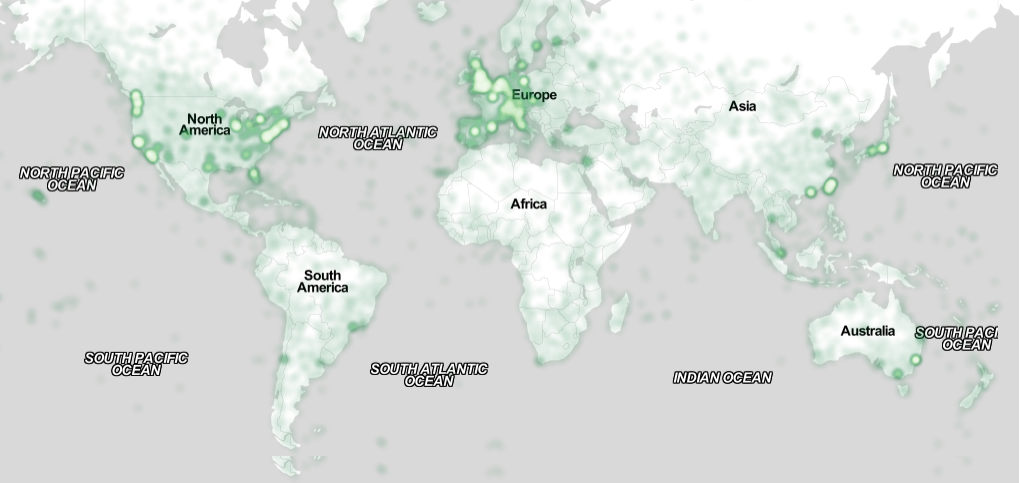
\includegraphics[width=1.75\columnwidth]{figures/map}
%  \caption{In this image, the map maximizes use of space. You can make
%    figures as wide as you need, up to a maximum of the full width of
%    both columns. Note that \LaTeX\ tends to render large figures on a
%    dedicated page. Image: \ccbynd~ayman on
%    Flickr.}~\label{fig:figure2}
%\end{figure*}

\section{Materiais e métodos}
Os protótipos da ferramenta \textit{e-Voz} foram desenvolvidos utilizando as tecnologias HTML5, JavaScript e CSS3, sendo posteriormente compilados para a plataforma Android por meio do \textit{framework} Apache Cordova~\cite{cordova:2016}. Para o experimento com usuários, foi utilizado um aparelho Motorola Moto G Dual SIM, com uma tela de 4,5 polegadas.

\subsection{Design experimental}
Para a verificação da hipótese aventada na Introdução, propusemos um teste A/B com os participantes entre os dois protótipos investigados, de modo que a única diferença visual entre ambos era o botão adicional de recursos estatísticos, presente na segunda versão [FIGURA X]. Desse modo, procurou-se minimizar a possibilidade de que outras variáveis relativas ao experimento tivessem algum impacto deletério sobre os resultados.

No teste proposto, os indivíduos deveriam completar a mesma tarefa com cada versão. Para reduzir vieses experimentais relativos ao aprendizado da tarefa, dividimos aleatoriamente os participantes em dois grupos: no primeiro, os indivíduos inciavam o experimento com o protótipo I e depois com o II, enquanto no segundo a ordem foi invertida. Ao final de cada tarefa, solicitava-se ao participante que respondesse a um questionário [TABELA X] com quatro questões cujas respostas foram dispostas em uma escala de Likert de cinco níveis~\cite{likert:1932}, com o intuito de verificar qual a experiência de usuário obtida.

Optou-se por realizar uma investigação inteiramente intra-sujeito e sem comparação com outras ferramentas equivalentes, a fim eliminar o viés de confirmação tipicamente presente em experimentos dessa natureza~\cite{dell:2012}. Após a conclusão das tarefas, uma entrevista semiestruturada deveria se realizada com cada participante a fim de identificar o cumprimento ou não de critérios de usabilidade, registrar os sentimentos relatados, investigar eventuais mudanças de comportamento na interação com cada protótipo e coletar opiniões gerais sobre a ferramenta.

\subsection{Protocolo experimental}
Todos os participantes se sujeitaram ao experimento em ambientes naturais. Ao ser abordado, o voluntário recebia informações sobre natureza da investigação, a garantia do experimentador de que todas as informações colhidas seriam confidenciais e o compromisso de que ele poderia desistir do experimento a qualquer momento que desejasse.

Uma vez de acordada sua participação, o experimentador exibia ao voluntário um dos protótipos da ferramenta \textit{e-Voz}, mostrando todas as suas telas e recursos interativos para que o participante pudesse se familiarizar com o aplicativo. Durante essa etapa, ele também era instruído sobre o contexto em que estava inserida a ferramenta e qual seria a natureza da tarefa requisitada, isto é, definir cinco problemas como prioritários dentre os 15 dispostos sobre o mapa do aplicativo com o intuito de auxiliar a Prefeitura de São Paulo na alocação de recursos públicos, utilizando ou não o botão de auxílio estatístico (no caso da versão II).

Enquanto o usuário selecionava os problemas que na sua opinião eram prioritários, o experimentador cronometrava o tempo gasto com a tarefa. Finda essa etapa, o participante recebia o questionário [XXX], para o qual lhe era informado explicitamente de que não havia tempo máximo para conclusão. Em seguida, a outra versão do protótipo lhe era apresentada, ressaltando a principal diferença em comparação com a anterior e, novamente, o usuário era instruído a realizar a mesma tarefa, que era cronometrada e, ao seu término, o mesmo questionário [XXX] era aplicado.

Concluída essa etapa, o experimentador solicitava ao participante mais alguns minutos para responder perguntas sobre a sua experiência com os protótipos. Durante a entrevista, foram feitas algumas questões abertas pré-definidas ao usuário [TABELA XXXX], bem como outras perguntas que o experimentador julgasse pertinente no contexto, tanto para clarificar uma resposta dada quanto para dirimir dúvidas sobre eventuais incoerências entre o comportamento observado pelo experimentador e o relatado pelo participante.



\section{Resultados}
- perfil dos participantes (idade, residência, sexo)\\
- estatísticas das respostas\\
- análise estatística\\
- tabelas com resultados\\


\section{Discussão}
Os dados reforçam a hipótese do viés de disponibilidade~\cite{tversky:1973} na tomada de decisão dos participantes. No grupo que interagiu primeiro com o protótipo I e depois com o II, nota-se uma alteração no critério de escolha da prioridade dos problema com o aumento de informações que subsidiam a tarefa. O mesmo não se observa no grupo que inicia a interação pelo protótipo II e depois segue para o I. Quando questionados sobre a mudança de postura, a maior parte dos participantes reconheceu utilizar um critério individualista quando não havia informações estatísticas disponíveis sobre a cidade, o que parece indicar que o recurso impacta positivamente para a tomada de decisões mais altruístas ou coletivistas.

\section{Limitações e trabalho futuro}
- quantidade de participantes\\
- utilizar meios e equipamentos informáticos faz que apenas parte da população, que tem acesso à essas tecnologias, possa contribuir, não abrangindo toda a população da cidade\\
- avaliação de outros fatures que contribuem para a interação colaborativa (rede social, por exemplo)\\
- avaliar se os recursos de gamification estimulam o usuário a usar mais a aplicação, e se em conjunto com a característica de rede social a aplicação continua sendo para resolver problemas da cidade ou se o propósito inicial se torna vago\\
- O quanto que essa mudança realmente impacta apenas será possível analisar com o tempo e a real implementação.

\section{Conclusão}
- oferecer recursos para melhora de decisão em plataformas colaborativas sem onerar a usabilidade de interfaces pode inicialmente ser um desafio, mas os efeitos aparentes tanto na qualidade da interação (percepção dos usuários) quanto na utilidade e resultados indicam um benefício significativo.


\section{Agradecimentos}

Agradecemos a todos os participantes que se submeteram voluntariamente ao experimento e aos nossos revisores, com seus comentários e críticas valiosas para o trabalho.


\balance{}


% BALANCE COLUMNS
\balance{}

% REFERENCES FORMAT
% References must be the same font size as other body text.
\bibliographystyle{SIGCHI-Reference-Format}
\bibliography{sample}

\end{document}

%%% Local Variables:
%%% mode: latex
%%% TeX-master: t
%%% End:
